\documentclass[letterpaper]{article}
\usepackage{amsmath, geometry, graphicx, tikz}
\usetikzlibrary{arrows.meta}
\bibliographystyle{plain}

\title{Variation of Genomic Imprinting in the Human Population,
and Analysis of its Sources and Psychiatric Consequences}
\author{Attila Guly\'{a}s-Kov\'{a}cs\(^\ast\), Ifat Keydar\(^\ast\),\\
Eva Xia, Menachem Fromer, Doug Ruderfer,\\
Ravi Sachinanandam, Andrew Chess}
\date{Mount Sinai School of Medicine}

\begin{document}
\maketitle

TODOs
\begin{enumerate}
\item check the fit of logi.S and filter out genes accordingly from the
regression analysis
\item plot terms of linear predictor using \texttt{termplot} in R
\item extend Fig.~\ref{fig:age-effect} with 3 additional panels: gender,
ancestry and Dx (psychiatric condition)
\item compare the effect of age from this work to that from
\cite{Perez2015} (Fig.~\ref{fig:mouse-comparison})
\item for the factor Dx set Control as reference level instead of AFF
\item randomly relabel individuals using the three levels of Dx and perform
regression
\item diminish size of plotting character for red symbols in
Fig.~\ref{fig:clusters} 
\item schematic figure on study design (Fig.~\ref{fig:study-design}) 
\item finish the rest of the Results section
\end{enumerate}

\newpage

\maketitle

\begin{abstract}
Lorem ipsum...
\end{abstract}

\section{Introduction}

Variation of expression level across genes, lifetime, cells, tissue types, as
well as individuals in the human population is clearly a major determinant of
phenotype REF.  A distinct, though related, question is the role of the
\emph{ratio} between maternal (or paternal) transcripts and those from both
alleles of a given gene.  Besides the random thermal fluctuations, which occur
in all genes, some genes display systematic \emph{parental bias} in allelic
expression.  The extreme form of this bias is known as monoallelic expression,
which may be non-random if expression is biased towards only one parent or
random otherwise \cite{Chess2012}.

Genomic imprinting is the classic, non-random, case of monoallelic expression,
which is mediated by epigenetic mechanisms that either concern single genes or
entire imprinted gene clusters~\cite{Peters2014,Plasschaert2014}.  Having
emerged late in evolution~\cite{Tucci2016}, imprinting of several genes have
been implicated in biological functions of mainly neurological, psychological,
behavioral and social type.  Mutations disrupting the expression of certain
imprinted genes are deeply penetrant causes of rare syndromes displaying
psychological, cognitive, and social dysfunction.  But it remains to be
established to what extent more subtle perturbations of parental bias might
contribute to common, highly polygenic psychiatric disorders such as
schizophrenia or autism.

Also of interest is how and why parental bias for a given imprinted gene
might vary between individuals.  Age is a prime candidate for regulator
given that several imprinted genes have been found to be functionally associated to either
perinatal stage (e.g.~suckling) or young adulthood (e.g.~maternal care).
Gender and ancestry are obvious further candidates.

A modern approach to study the variation of parental bias is to differentiate
maternal and paternal transcripts based on those single nucleotide
polymorphisms (SNPs) that contribute to the heterozygosity of a given
individual and gene.  Coupled with high throughput techniques such as RNA-seq
this approach permits the quantification of both genome-wide and
among-individual variation.  Several research groups
\cite{Gregg2010a,Perez2015,DeVeale2012} combined this approach with F1 hybrids
of crossed mouse strains and found, for instance, that \(\approx 1\%\) of all
genes are imprinted, although some \cite{Perez2015} of the same researchers
previously estimated \(> 5\%\), leaving this question controversial.
Another finding is the differential effect of age, but not gender, on parental
bias: shifting from neonatal age to young adulthood down-regulated bias in
ca.~\(20\%\) of detected imprinted genes, up-regulated in \(6\%\) and had no
effect on the remaining nearly \(75\%\).

While such designed mouse experiments afford high statistical power their
relevance is at best unclear to human neuropsychological function, ageing and
ancestry.  The present work directly addresses these points by utilizing
post-mortem tissue samples from the dorsolateral prefrontal cortex (DLFPC)
from nearly 600 individuals of different age, psychiatric condition, and
ancestry, and by performing the RNA-seq based quantification of parental bias.

\section{Methods}

\subsection{Brain samples}

\footnote{This and the following two subsections
have been taken apart from a few minor modifications, literally from Ifat's
version of the manuscript.  They require double-checking because I was not
involved with the work described in them.}

Human RNA samples were collected from the dorsolateral prefrontal cortex of
the CommonMind consortium (CMC), from a total of \(579\) individuals after
quality control. Subjects included 267 control individuals, as well as 258
with schizophrenia (SCZ) and 54 with affective spectrum disorder (AFF).
RNA-seq library preparation uses Ribo-Zero (which selects against ribosomal
RNA) to prepare the RNA, followed by Illumina paired end library generation.
RNAseq was performed on Illumina HiSeq 2000.

\subsection{RNA-seq, mapping and SNP calling}

We mapped 100bp, paired-end reads (\(\approx50\) million reads per sample) using Tophat
to Ensembl gene transcripts of the human genome (hg19; February, 2009) using
default parameters with 6 mismatches allowed per pair (200bp total). We
required both reads in a pair to be successfully mapped and we removed reads
that mapped to \(>1\) genomic locus. Then, we removed PCR replicates using the
Samtools rmdup utility; around one third of the reads mapped (which is
expected, given the parameters we used and the known high repeat content of
the human genome). We used Cufflinks to determine gene expression of Ensembl
genes, using default parameters. Using the BCFtools utility of Samtools, we
called SNPs (SNVs only, no indels). Then, we invoked a quality filter
requiring a Phred score \(>20\) (corresponding to a probability for an
incorrect SNP call \(<0.01\)).

We annotated known SNPs using dbSNP (dbSNP 138, October 2013). Considering all
579 samples, we find 936,193 SNPs in total, 563,427 (60\%) of which are novel.
Further filtering of this SNP list removed the novel SNPs and removed SNPs
that either did not match the alleles reported in dbSNP or had more than 2
alleles in dbSNP. We also removed SNPs without at least 10 mapped reads in at
least one sample. Read depth was measured using the Samtools Pileup utility.
After these filters were applied, 364,509 SNPs remained in 22,254 genes. These
filters enabled use of data with low coverage, as described below. For the 579
samples there are 203 million data points (reads overlapping one of the
364,509 SNPs defined above), of which 158 million (78\%) have genotype data
available (array or imputation), which is used later in the pipeline.

\subsection{Genotyping and calibration of imputed SNPs}

DNA samples were genotyped using the Illumina Infinium SNP array. We used
PLINK with default parameters to impute genotypes for SNPs not present on the
Infinium SNP array using 1000 genomes data. To maximize the number of genes
assessable for monoallelic expression, while minimizing false positive
monoallelic expression calls which can arise if the underlying SNP has been
incorrectly called as heterozygous by the imputation, we calibrated the
imputation parameters.

We first examined how many SNPs were heterozygous in DNA calls and had a
discordant RNA call (i.e. homozygous RNA-SNP call) using different imputation
parameters. Known imprinted genes were excluded. We examined RNA-seq reads
overlapping array-called heterozygous SNPs which we assigned a heterozyous
likelihood value, \(L_\mathrm{het}\) of 1, separately from RNA seq data
overlapping imputed heterozygous SNPs, where \(L_\mathrm{het}\) values could
range from 0 to 1. Based on iterative examination with different thresholds,
we selected a \(L_\mathrm{het}\) cutoff of 0.95 (i.e. imputation confidence
level of 95\%), and a minimal coverage of 7 reads per SNP. With these
parameters, the discordance rate (monoallelic RNA genotype in the context of a
heterozygous DNA genotype) was 0.71\% for array-called SNPs and 3.2\% for
imputed SNPs.

While undoubtedly, a portion of the excess of discordance for the imputed SNPs
is due to imputation error, downstream parts of analytic pipeline are designed
taking into account the possibility of imputation error, as described below.
One key is that for most genes there are multiple imputed SNPs and we consider
data for all of them. Another key is that if even one SNP has evidence for
biallelic expression (whether or not there is imputation data), we exlcude
that individual due to the conflict. At this point, the matrix includes 147
million data points covering 213,208 SNPs, of which 114 million (77\%) have
imputation data.

\subsection{The read count ratio and related quality filtering}

\label{sec:filtering}

The central quantity of this work is an \(m\times n\) matrix of read count ratios
\(\mathbf{S} = [S_{ig}]_{ig};\; i=1,...,m; \; g\in\mathcal{G}\), where
\(m=579\) is the number of individuals and \(n\) is the number of genes
in a set \(\mathcal{G}\) of unfiltered or filtered genes (\(n=15584\) and \(5307\),
respectively).  The read count ratio for
individual \(i\) and gene \(g\) is defined as
\begin{equation}
S_{ig} = \frac{H_{ig}}{T_{ig}}= \frac{\sum_s H_s}{\sum_sT_s},
\label{eq:S-definition}
\end{equation}
where the summation runs through all heterozygous SNPs \(s\) that occur in
\((i,g)\).  The statistic \(H_s\) and \(T_s\) in Eq.~\ref{eq:S-definition} are
the higher and total RNA-seq read count at SNP \(s\); \(H_s\) is higher in the
sense that if the alleles at \(s\) are \(a,b\) and the corresponding read counts
\(X_a,X_b\), then \(H_s = X_a\) if \(X_a\ge X_b\) and \(H_s = X_b\) otherwise.
The total read count is simply \(T_s = X_a + X_b\).

Two kind of data filters were applied sequentially: (1) a \emph{read count-based}
and (2) an \emph{individual-based}.  The read count-based filter removes any
such pair $(i,g)$ of individual $i$ and genes $g$ for which the total read
count $T_{ig}<t_\mathrm{rc}$, where $t_\mathrm{rc}$ is the read count
threshold and was set to 15. The individual-based filter removes any genes $g$ (across all
individuals) if read count data involving $g$ are available on less than
$t_\mathrm{ind}$ number of individuals, set to 25.
These filtering procedures were preceded by an initial read count-based
filter, which removed each combination \((i,s)\) of individual \(i\) and SNP
\(s\) for which fewer than 7 reads had quality score \(\ge20\).  After the
initial filtering the number of genes was \(n=15584\), which decreased to
\(n=5307\) after the final, individual-based, filtering step.

The test for nearly unbiased expression of parental transcripts was defined by
the criterion
\begin{equation}
S_{ig} \le 0.6 \text{ and } \mathrm{UCL}_{ig} \le 0.7,
\label{eq:unbiased-test}
\end{equation}
where the 95\% upper confidence limit was calculated from a normal approximation to
likelihood:
\begin{equation}
\mathrm{UCL}_{ig} = S_{ig} + z_{0.975} \sqrt{\frac{S_{ig} (1 - S_{ig})}{T_{ig}}},
\end{equation}
such that $z_{p}$ is the $p$ quantile of the standard normal distribution and
$T_{ig}$ is, as before, the total read count.

\subsection{Regression models to explain population-wide variation}
\label{sec:methods-regression}

Let \(m\) denote the number of individuals/samples and \(\mathcal{G}\) the set
of \(n=5307\) genes that passed quality filtering.  Regression analysis
involved a subset \(\mathcal{G}_1\subset\mathcal{G}\) of \(n_1=30\) genes
called as imprinted.

The basic model, unlm.S, is
\begin{eqnarray}
\mathbf{S} &=& \mathbf{X} \boldsymbol{\beta} + \boldsymbol{\varepsilon},
\label{eq:unlm.S-matrix-form} \\
\varepsilon_{ig} &\overset{\mathrm{iid}}{\sim}& \mathrm{Norm}(0, \sigma^2_g)
\end{eqnarray}
where the response \(\mathbf{S}\) is an \(m\times n_1\) matrix of read count ratios,
\(\mathrm{X}\) is an \(m\times p\) design matrix, \(\boldsymbol{\beta}\) is a \(p\times n_1\) matrix of regression
coefficients~(Table~\ref{tab:predictors}), the random error \(\boldsymbol{\varepsilon}\) has the same
dimension as \(\mathbf{S}\), and gene \(g\in \mathcal{G}_1\).  Eq.~\ref{eq:unlm.S-matrix-form} may be given as
\begin{equation}
S_g = \mathbf{X} \beta_g + \varepsilon_g,
\label{eq:unlm.S-vector-form}
\end{equation}
where the vectors \(S_g, \beta_g, \varepsilon_g\)
are single columns taken from their respective matrix counterparts.

unlm.S was extended in several ways, yielding
\begin{enumerate}
\item four normal linear models unlm.S, unlm.R, wnlm.S, wnlm.S
\item two logistic models logi.S and logi2.S.
\end{enumerate}

The general form of the four normal linar models
(cf.~\ref{eq:unlm.S-vector-form}) is
\begin{equation}
\mathbf{W}_g^{1/2} \tau(S_g) = \mathbf{W}_g^{1/2} \mathbf{X} \beta_g + \varepsilon_g.
\label{eq:nlm-general}
\end{equation}
The extension here consists of \(\mathbf{W}_g\), an \(m\times m\) diagonal matrix of
weights \(w_{ig}\) on the \(i\)-th diagonal position, and \(\tau\), a
transformation on read counts.  These quantities specify the four normal
linear models as laid out in Table~\ref{tab:nlm}.

\begin{table}
\begin{center}
\begin{tabular}{c|cc}
model & transformation \(\tau\) & weights \(w_{ig}\) \\
\hline
unlm.S & none & 1 \\
unlm.R & rank transf. & 1 \\
wnlm.S & none & \(T_{ig}\) \\
wnlm.R & rank transf. & \(T_{ig}\) \\
\end{tabular}
\end{center}
\caption{Specificiation of four normal linear models based on read count
transformation \(\tau\) and weights \(w_{ig}\).}
\label{tab:nlm}
\end{table}

The logistic models, logi.S or logi2.S, share the general form
\begin{eqnarray}
S_g &=& \mu_g + c\, \varepsilon_g
\label{eq:logi-general}
\\
\mu_g &=& h(\mathbf{X} \beta_g) \\
\varepsilon_{ig} + \mu_g &\overset{\mathrm{iid}}{\sim}& \mathrm{Binom}(\mu_g, T_{ig}).
\label{eq:binom-error}
\end{eqnarray}
The link function \(h\) is \(h(u) = e^u / (1 + e^u)\) for logi.S and \(h(u) =
e^u / (2 + 2e^u)] + 1/2\) for logi2.S, and the scaling constant \(c=\) 1
 and \(1/2\), respectively.  Thus, the response \(S_g\) under logi2.S is scaled and shifted relative to
that under logi.S such that (with probabilty one) \(1/2\le S_{ig}\le 1\) under the former and
\(0\le S_{ig}\le 1\) under the latter.

Each of the six models has \(p\times n_1\) regression parameters corresponding to the
dimension of \(\boldsymbol{\beta}\).  This allows different behavior for
different genes since \(\beta_1\neq ...\neq\beta_{n_1}\) in general.
Therefore, the estimated regression coefficients are reported as \(\hat{\beta}_g =
(\hat{\beta}_{1g},...,\hat{\beta}_{jg},...,\hat{\beta}_{pg})\) for each gene \(g\), often
replacing index \(j\) with the name of the parameter such as \emph{Age} or
\emph{InstitutionPitt}.

A second set of six models was also
fitted, for which \(\boldsymbol{\beta}\) was constrained such that \(\beta_1 =
... = \beta_{n_1}\).  This was achieved by aggregating over genes
\(g\in\mathcal{G}_1\) the higher read count \(H'_i = \sum_g H_{ig}\), the
total read count \(T'_i = \sum_g T_{ig}\), redefining the read count ratio
as \(S'_i = H'_i / T'_i\), and replacing \(S_g\) by \(S'=(S'_1,...,S'_m)\) in
Eq.~\ref{eq:unlm.S-vector-form},~\ref{eq:nlm-general},~\ref{eq:logi-general}, and \(T_{ig}\) by \(T'_i\) in
Table~\ref{tab:nlm} and Eq.~\ref{eq:binom-error}.  Note that such aggregation
simplifies the matrix variables in Eq.~\ref{eq:unlm.S-matrix-form} to the
corresponding vector variables in Eq.~\ref{eq:unlm.S-vector-form}.  Because \(S'_i\) is a
weighted average of \(\{S_{ig}\}_i\), results under these models are reported
as \(\hat{\beta}_\mathrm{WA} =
(\hat{\beta}_{1\mathrm{WA}},...,\hat{\beta}_{j\mathrm{WA}},...,\hat{\beta}_{p\mathrm{WA}})\).  A
third set of models is a slight variation of this second set in that
aggregation was done on a smaller subset of 8 genes selected at the initial
stage of the study.  Under these models the results are reported using the
WA.8 subscript instead of WA.

These \(3\times 6\) models are all multiple regression ones with \(p<1\)
parameters.  Three corresponding sets of models with a single Age parameter
(\(p=1\)) were also fitted but the results were only used for graphical
comparison of model fits in terms of predictions
Fig.~\ref{fig:predicted-curves} but not for quantitative inference.

\section{Results}

\subsection{Study design}

The genome- and population-wide variation of parental bias was assessed using
DLPFC tissue samples, one from each of \(m=579\) study individuals
\(i=1,...,m\)~(Fig.~\ref{fig:study-design}).
For each combination \((i,g)\) of individuals and \(15584\) genes
\(g\in\{g_1,...,g_{15584}\}\) (which passed an initial quality filter, see
Section~\ref{sec:filtering}) the set
of all heterozygous SNPs was identified with SNP-array genotyping, and
expression was quantified at each SNP separately for the two alleles by
counting RNA-seq reads noting the allele associated with the \emph{higher read
count} (as opposed to the \emph{lower read count}).  For a given \((i,g)\)
combination higher and lower read counts were then separately aggregated
across the heterozygous SNPs yielding the statistics \(H_{ig}\) and
\(L_{ig}\), as well as the \emph{total read count} \(T_{ig} = H_{ig} +
L_{ig}\).  Genes were then quality filtered based on the conditional
distribution of total read count across the 579 individuals for any given
gene, leaving \(n=5307\) genes in the analysis.  The \emph{read count ratio}
statistic, defined as \(S_{ig} = H_{ig}/T_{ig}\), was used to quantify
parental bias towards the more highly expressed parental allele (see also
Eq.~\ref{eq:S-definition} in Section~\ref{sec:filtering}).

\begin{figure}
\begin{center}
\includegraphics[width=0.6\textwidth]{figures/mona_1.png}
\end{center}
\caption{TODO: Study design.  This figure (if deemed useful) will
schematically illustrate variation of parental bias across a few genes by
showing several maternal and paternal transcripts, and will also demonstrate
technical sources of variation by depicting
the corresponding RNA-seq read counts at heterozygous SNPs.  Showing variation across
individuals would be desirable but would complicate figure.}
\label{fig:study-design}
\end{figure}


Taking a genome-wide viewpoint, it is helpful to regard the read count ratio
as a set of random variables \(\{S_{g_1},...,S_{g_n}\}\), each of which varies
across the human population described by its own distribution.  The difference
(or similarity) among the corresponding set of distributions is an indicator
of biological mechanisms that differentiate genes' parental bias.  For any
given gene \(g\) the observed \(S_{1g},...,S_{mg}\) from the present data on
\(m\le579\) individuals estimates the distribution of \(S_g\).  That
distribution, in turn, informs us on further biological mechanisms that
differentiate individuals' parental bias for that gene but at the same time
also reflects variation of \(S_g\) that arise from technical sources.

\begin{table}
\begin{center}
\begin{tabular}{r|l}
predictor & parameter(s)\\
\hline
Age & Age\\
Institution & [MSSM], Penn, Pitt\\
Gender & [Female], Male\\
PMI & PMI\\
Dx & [AFF], Control, SCZ\\
RIN & RIN\\
RIN2 & RIN2\\
RNA\_batch & [0], A, B, C, D, E, F, G, H\\
Ancestry.1 & Ancestry.1\\
\vdots & \vdots \\
Ancestry.5 & Ancestry.5\\
\end{tabular}
\caption{Variables used as predictors of read count ratio for the study of
regulation and consequences of parental bias.  The right column lists the
corresponding regression parameters and, in square brackets [ ], the baseline
level against which other levels are contrasted.  PMI: post-mortem interval; Dx:
disease status; AFF: affective spectrum disorder; SCZ: schizophrenia; RIN: RNA
integrity number; RIN2: the square of RIN; Ancestry.\(k\): the \(k\)-th
eigenvalue from the decomposition of genotypes indicating population structure}
\label{tab:predictors}
\end{center}
\end{table}

Besides the genomic measurements leading to read count ratios our data include
observations on variables (Table~\ref{tab:predictors}) that we found (see
Section~\ref{sec:results-regression} below) to be informative for the genome-wide
dissection of various biological mechanisms and technical effects underlying
the observed variation of read counts.  We carried out a theoretical
study\footnote{I wonder if we should attach my modeling article confidentially
for the reviewers.  See that article
at:\\http://bernie.anbg.mssm.edu/\~{}attila/assets/projects/monoallelic-brain/2016-04-14-braim-model.pdf}
that culminated in several probabilistic models of read counts---even at
individual SNPs---and other observed variables (Fig.~\ref{fig:agk}).  These
models may successfully capture the observed complex pattern of correlations
among the measured variables (Section~\ref{sec:results-regression}); but our
theoretical work also showed that their computational implementation and
evaluation of their properties and performance in relevant tasks would reach
far beyond the present scope.  Therefore, we decided to resort to relatively
simple conventional models, some of which were found to fit reasonably well to
allow quantitative inferences on the small subset of genes called imprinted
(Section~\ref{sec:results-regression}).  On the genome-wide scale (next section) we
present only an exploratory statistical analysis, which none-the-less permits
qualitative conclusions under careful interpretation.

\subsection{Genome- and population-wide variation of parental bias}

\begin{figure}
\begin{center}
\includegraphics[scale=0.6]{figures/2016-07-19-genome-wide-S/complex-plot-1.png}
\end{center}
\caption{}
\label{fig:ranking-genes}
\end{figure}

The top three plots of Fig.~\ref{fig:ranking-genes} all show the empirical distribution
of \(S_\mathrm{PEG10}, S_\mathrm{ZNF331}\) and \(S_\mathrm{AFAP1}\), where
PEG10 and ZNF331 are \emph{known imprinted genes} based on prior evidence and
AFAP1 is referred to as \emph{candidate gene} as it lacks such evidence.  For
all three genes \(S_g\) varies greatly within its theoretical range
\([\frac{1}{2}, 1]\).  This variation is attributable to both technical and biological effects
and is consistent with substantial population-wide variation of parental bias.

The probability density of \(S_g\) for the two known imprinted
genes is shifted towards the theoretical maximum (relative to the density of
the candidate gene), which indicates near monoallelic expression in a great
fraction of individuals for these two genes.  This is expected if \(S_g\) is
indeed a useful estimator of the relative level of maternal (or paternal,
whichever is greater) transcripts.  But the shift is clearly
stronger for PEG10 than for ZNF331, suggesting quantitative differences even
among imprinted genes.  This motivated the ranking of all 5307 genes
based on a gene score that quantifies the shift in distribution.  We defined the score of
gene \(g\) as the fraction of individuals with \(S_{ig}>0.9\); as the filled green
circles show in Fig.~\ref{fig:ranking-genes} this is equivalent to 1 less the
empirical distribution function (ECDF), evaluated at \(0.9\) (the second and
third plots from the top of Fig.~\ref{fig:ranking-genes}).

The lower half of Fig.~\ref{fig:ranking-genes} shows the distribution of
\(S_{g_1},...,S_{g_{n}}\) ordered by rank from the top (rank 1) to bottom
(rank 5307).  Although the distributional shift is gradual from the top ranking
\(g_1=\mathrm{MAGEL2}\) to the lowest ranking genes,
Fig.~\ref{fig:ranking-genes} provides a visual argument that the fraction of
imprinted genes is no more than \(1\%\) of all genes.

\begin{figure}
\begin{center}
\includegraphics[scale=0.6]{figures/2016-08-01-ifats-filters/top-ranking-genes-1.pdf}
\caption{}
\label{fig:top-genes}
\end{center}
\end{figure}

Consistent with previously described imprinted gene clusters the top-scoring
genes tend to cluster according to genomic position (Fig.~\ref{fig:clusters})
and most, but not all, of them are known imprinted genes
(Fig.~\ref{fig:top-genes}).  The high scoring candidates were classified on
the basis of their distance from known imprinted gene clusters as nearby and
distant candidates; the former class was taken as novel imprinted genes and
the latter as false positives by considering the epigenetic nature of
imprinting mechanisms and the typical, MB-scale, length of those epigenetic
marks.  Besides this mechanistic argument, the fraction of individuals passing
a statistical test for the nearly unbiased expression of alleles
(Eq.~\ref{eq:unbiased-test}) also supports this classification, as shown by
the black bars in Fig.~\ref{fig:top-genes}. Conversely, more than a third of
all known imprinted genes (within the 5307-sized gene set) score low.  As the
known imprinted genes were identified in different tissue types and organisms,
these results indicate the context-dependence of imprinting.

\begin{figure}
\begin{center}
\includegraphics[scale=0.6]{figures/2016-06-26-trellis-display-of-data/S-age-gender-1.png}
\caption{}
\label{fig:S-age-gender}
\end{center}
\end{figure}

\subsection{Sources and psychological consequences of variation}
\label{sec:results-regression}

We selected the 27 top-scoring genes in the ``known imprinted'' and ``nearby
candidate'' categories shown in blue and green in Fig.~\ref{fig:top-genes} and
added three more known imprinted genes (NLRP2, IGF2 and UBE3A) that scored
reasonably high (Fig.~\ref{fig:known-genes}).  The sources and psychological
consequences of the variation of parental bias in these 30 genes was analyzed
further through the detailed characterization how the read count ratio depends
on the biological and technical variables---i.e.~the predictors---listed in Table~\ref{tab:predictors}.

Fig.~\ref{fig:S-age-gender} shows patterns of dependence (or independence) of
the read count ratio \(S_g\) for a given gene \(g\) on age and gender.  From
this visual inspection it seems that for several genes age is informative to
the distribution of \(S_g\) in terms of both the location (e.g.~the mean of
\(S_g\)) and scale (e.g.~variance); such apparent dependence on gender is not
clear.

This qualitative result, however, is greatly complicated by the association
among predictors: taking only pairwise associations the situation is already
complex given the observed strong association between age and gender with each
other and with many other predictors (Fig.~\ref{fig:predictor-associations})
but higher order associations might also exist in the data.
The correct interpretation of plots like Fig.~\ref{fig:S-age-gender} also depends on
the amount of data, i.e.~the total read count \(T_{ig}\), based on which the
read count ratio \(S_{ig}\) was calculated.  Fig.~\ref{fig:weight-of-evidence}
shows how \(T_{ig}\) varies both within a gene and across genes.

\begin{figure}
\begin{center}
\includegraphics[scale=0.6]{figures/2016-08-23-glm-sampling-distributions/GRB10-1.png}
\end{center}
\caption{}
\label{fig:predicted-curves}
\end{figure}

These considerations motivated us to fit various generalized linear regression
models, one for each gene, by treating read count ratio as response and the
variables in Table~\ref{tab:predictors} as predictors. The thick black curves
and colored strips in Fig.~\ref{fig:predicted-curves} represent the predicted
read count ratio and prediction intervals, respectively, under four of these
models for the gene GRB10.  To allow visual evaluation of model fit to the
observed values (green dots) the only predictor is age for the all models in
these plots but for quantitative statistical inference all predictors were
included.

As indicated by Fig.~\ref{fig:predicted-curves}, the logistic models logi.S
and logi2.S fitted for most genes much better to the data than various flavors
of normal linear models such as wnlm.S.  This is because only the former could
express the observed steep dependence of the response's variance on its
average.  Scale--location plots (for instance
Fig.~\ref{fig:non-constant-variance}, top left) confirmed the poor fit of
normal linear models, and calculated Cook's distances revealed also a
non-systematic variation in error variance
(Fig.~\ref{fig:non-constant-variance}, top right).  Both the systematic and
non-systematic variation was remedied by rank transformation of observed read
count ratios leading to the wnlm.R model
(Fig.~\ref{fig:non-constant-variance}, bottom left and right) but this came at
the price of a large increase in the overall error variance relative to the
variation by wnlm.R (Fig.~\ref{fig:predicted-curves}).  Based on these results
the wnlm.S models were deemed inadequate excluded from further
analysis.

Since all of these models account for each predictor separately, they are
expected, in principle, to successfully dissect their effects although the
observed association among the predictors might adversely affect parameter
estimation due to collinearity.  Inspection of likelihood surfaces suggested
that perhaps with the exception of those including the predictor RIN, the
associations only moderately distort likelihood surfaces
(Fig.~\ref{fig:likelihood-surface}).

That logistic models fit the data relatively better was suggested by not only plots
similar to Fig.~\ref{fig:predicted-curves} but also the fact that these are natural
models of count data, which readily account for the observed variation of
total read count, while normal linear models in general do not.  Therefore we
used weighted normal linear models (i.e.~wnlm.R) in addition to unweighted
ones (unlm.R), where the weight of observation on individual \(i\) was given
by total read counts \(T_{ig}\) (Table~\ref{tab:nlm}).  In addition, we fitted
a variant of each model (denoted as ``.WA'') which assumes that predictors
affect read count ratio for each gene identically (see
Section~\ref{sec:methods-regression}).

Fig.~\ref{fig:all-effects-logi.S},~\ref{fig:all-effects-logi2.S},~\ref{fig:all-effects-wnlm.R},
and~\ref{fig:all-effects-unlm.R} present the estimated regression coefficients
along with their 99\% confidence intervals for all of the above models.  The
more significant results under logistic models indicated that they were indeed
more powerful than the weighted or unweighed normal linear models, in
agreement with their better fit and favorable theoretical properties and that
they avoid the loss of information incurred by rank transformation.  But it
must be added to this conclusion that logistic models might also be more prone
to bias because much of their predicted sigmoidal curve was extrapolated from
the data (Fig.~\ref{fig:predicted-curves}).  Results were very similar under
the two logistic models.  Moreover, the great variation of regression
coefficients across genes suggested that the ``.WA'' models were inadequate
because predictors likely affect genes differentially.  These findings made us
give priority to the logi.S model and use wnlm.R mainly to check the results'
consistency under these two models.

The effects of four biological predictors---age, gender, ancestry and
psychiatric condition---on read count ratio of individual genes are depicted
in Fig.~\ref{fig:age-effect}.

TODO: finish the rest of the Results section.

\begin{figure}
\begin{center}
\includegraphics[scale=0.6]{figures/2016-08-08-imprinted-gene-clusters/segplot-1.pdf}
\end{center}
\caption{This figure will be extended with 3 additional panels: gender,
ancestry and Dx (psychiatric condition)}
\label{fig:age-effect}
\end{figure}

\begin{figure}
\begin{center}
\includegraphics[scale=0.6]{figures/2016-06-22-extending-anova/anova-effects-fw-rv-logi-S-1.pdf}
\end{center}
\caption{}
\label{fig:anova}
\end{figure}

\begin{figure}
\begin{center}
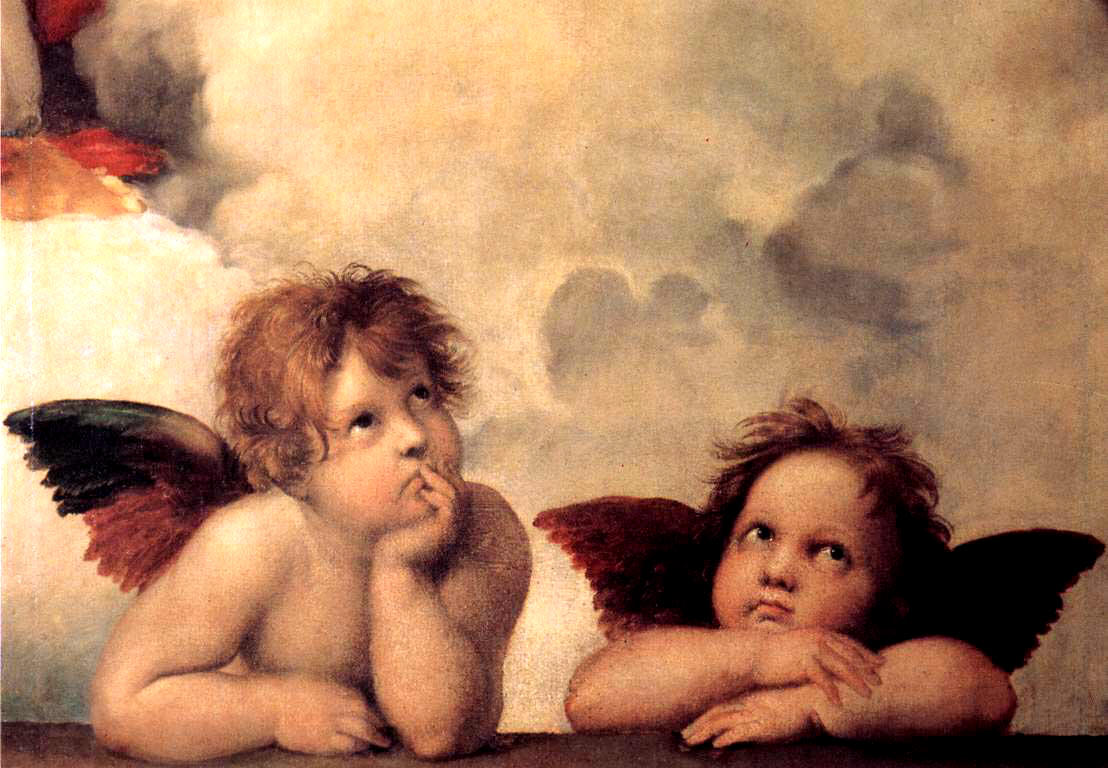
\includegraphics[width=0.6\textwidth]{figures/raffaello-putti.jpg}
\end{center}
\caption{TODO: Comparison of the effects of age between the present work and a
previous mouse study~\cite{Perez2015}.  This figure would either be presented
in the main or supplementary material depending on how conclusive the result
is.}
\label{fig:mouse-comparison}
\end{figure}


\section{Discussion}

The main results of this work may be interpreted in terms of the scheme in
Fig.~\ref{fig:scheme}.  The scheme presents all \(n\) imprinted genes in a
tissue, such as the DLPFC, which is relevant to neural function.  Parental
bias is putatively regulated by age, gender, ancestry, and possibly other
biological factors.  The nature of regulation---simple up- or down-regulation,
no effect, or some more complex pattern---is captured in the functions
\(\psi_1,...,\psi_n\).  Function \(\phi\) maps jointly the \(n\) parental
biases to neuropsychology, and connects therefore the molecular phenotypic
level to the organismal one.

\begin{figure}[h]
\begin{center}
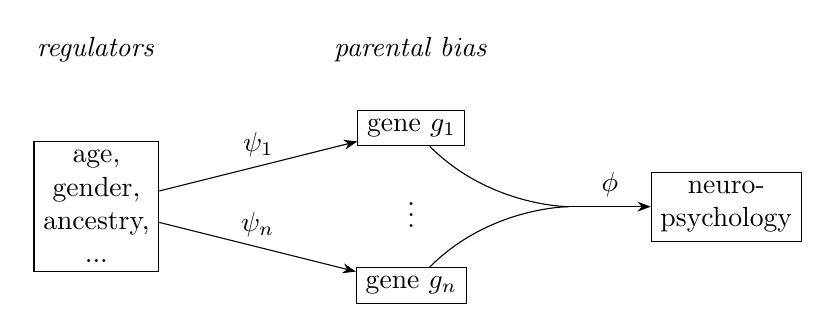
\begin{tikzpicture}[align=center]
\node at (-4,2) {\emph{regulators}};
\node[draw] (A) at (-4,0) {age,\\gender,\\ancestry,\\...};
\node at (0,2) {\emph{parental bias}};
\node[draw] (G1) at (0,1) {gene \(g_1\)};
\node at (0,0) {\vdots};
\node[draw] (Gn) at (0,-1) {gene \(g_n\)};
\coordinate (C) at (2,0);
\node[draw] (B) at (4,0) {neuro-\\psychology};
\draw[-Stealth] (A) -- node[anchor=south] {\(\psi_1\)} (G1);
\draw[-Stealth] (A) -- node[anchor=south] {\(\psi_n\)} (Gn);
\draw[-Stealth] (C) -- node[anchor=south] {\(\phi\)} (B);
\draw (G1) .. controls (1,0) and (2,0) .. (C);
\draw (Gn) .. controls (1,0) and (2,0) .. (C);
\end{tikzpicture}
\end{center}
\caption{}
\label{fig:scheme}
\end{figure}

Our genome-wide analysis suggests that \(<1\%\) of all genes are imprinted,
which implies \(n\approx 200\).  This provides evidence, in addition to
previous similarly conservative estimates of \(n\)
\cite{Perez2015,DeVeale2012}, against the controversial estimate of \(n\approx
1300\) \cite{Gregg2010a}.

More interestingly, we find that several regression coefficients differ
significantly from zero, which suggests that age, gender and ancestry do
indeed regulate parental bias in at least some imprinted genes in the human
DLPFC.  We infer that these three regulators exert gene-specific effects, up-
or down-regulating parental bias in a subset of imprinted genes while having
no (detectable) impact on the rest.  That these predictors differ in the
subset of genes they affect significantly hints at the potential complexity of
regulation.  A further layer of that complexity arises from possible
interactions among these predictors, which is in fact consistent with the
dependence of the age effect on gender in our conditional analysis.

The interpretation of the present results as the effect of (human) ancestry on
parental bias points to genetic regulatory mechanisms of imprinting that
modulate the known epigenetic mechanisms.  Given the late emergence of
imprinting in therian phylogeny and its role in neuropsychological and social
function, the genetics of parental bias may well be an increasingly important
target of natural selection.  Also, the ancestry effect is a remarkable
novelty of our work since previous studies, all using in-bread mouse strains,
failed to address this point.  As for age, a similar differential effect was
found in the mouse cerebellum to the effect we observe here. Gender, however,
had no significant effect in the same mouse study.

The above interpretation certainly depends on our statistical inference, which
in turn is based on the present data and regression models, both of which have
serious limitations.  Some of these---related to differing sequencing and
genotyping protocols---might be alleviated by improved across-institute
standardization.  But others, such as the confounding of age by certain
technical variables (e.g.~institution), are hopelessly entangled with the
observational nature of post mortem human studies, which precludes orthogonal,
that is clearly interpretable, decomposition of the variation of the observed
measure of parental bias (the response) into separate technical and biological
components.  In addition, non-orthogonality also limits statistical power.  But even
if the data fulfilled orthogonality, the present regression models would still
remain too rigid to account for the relative overdispersion of RNA-seq read
counts, the uncertainty surrounding haplotype, and that genes are neither
completely independent nor completely identical in their parental bias.  In
future work these ought to be tackled either with recently developed
hierarchical models built on normal linear model \cite{Perez2015,Law2014} or,
if regulators indeed strongly interact as the present work indicates, by the
adoption of Bayesian networks.

The molecular mechanism mediating the age effect.  TODO: clusters and regression
coefficients for gender and ancestry

Even if the regulatory effect of age, gender, ancestry, etc, on parental bias
is more firmly established by methodological improvements and more data, it
still remains to be determined whether (and how) the corresponding changes in
expression phenotype affect neural and psychological properties and might be
causal to some common psychiatric disorders.  This work may be considered an
initial step towards that aim as the estimated regression coefficients,
associated with SCZ or AFF, provide statistically weak hints at that
causality.

A more general question is how function \(\phi\) in Fig.~\ref{fig:scheme}
integrates parental bias across genes and maps that signal to organismal
phenotype.  That mapping occurs through the intermediate domain of cellular
metabolism.  Therefore, extending the present ``multi-omic'' data collection
with a metabolic layer appears promising, especially because rather specific
metabolism characterizes several imprinted genes \cite{Tucci2016,Peters2014}.
Adopting single-cell RNA-seq in the present framework would be another
interesting extension that could possibly elucidate the role of random
monoallelic expression.

In fact, the question regarding the map \(\phi\) is even more general, since
it is plausible that parental bias acts jointly with overall expression level
(this is not indicated in Fig.~\ref{fig:scheme}).  If so, the resolution of
the prevailing system biology is to be refined from mere genes to separate
maternal and paternal copies.  On the other hand, the present finding that
parental bias substantially varies across individuals even withing the same
tissue calls for a conceptual shift from the current practice of regarding
genes unconditionally as either imprinted or not to considering instead the
conditional distribution of their parental bias within the population given
regulators such as age, gender, and ancestry.

\bibliography{monoall-ms}

\section{Supplementary Material}

\newpage

% Supplementary figures

\setcounter{figure}{0}
\makeatletter 
\renewcommand{\thefigure}{S\@arabic\c@figure}
\makeatother

\begin{figure}
\begin{center}
\includegraphics{figures/by-me/monoall-M1}
\hspace{\fill}
\includegraphics{figures/by-me/monoall-M2}
\end{center}
\caption{AGK models: M1 (left) and M2 (right)}
\label{fig:agk}
\end{figure}

\begin{figure}
\begin{center}
\includegraphics[scale=0.6]{figures/2016-08-08-imprinted-gene-clusters/score-genomic-location-1.png}
\end{center}
\caption{}
\label{fig:clusters}
\end{figure}

\begin{figure}
\begin{center}
\includegraphics[scale=0.6]{figures/2016-08-01-ifats-filters/known-genes-1.pdf}
\caption{}
\label{fig:known-genes}
\end{center}
\end{figure}

\begin{figure}
\begin{center}
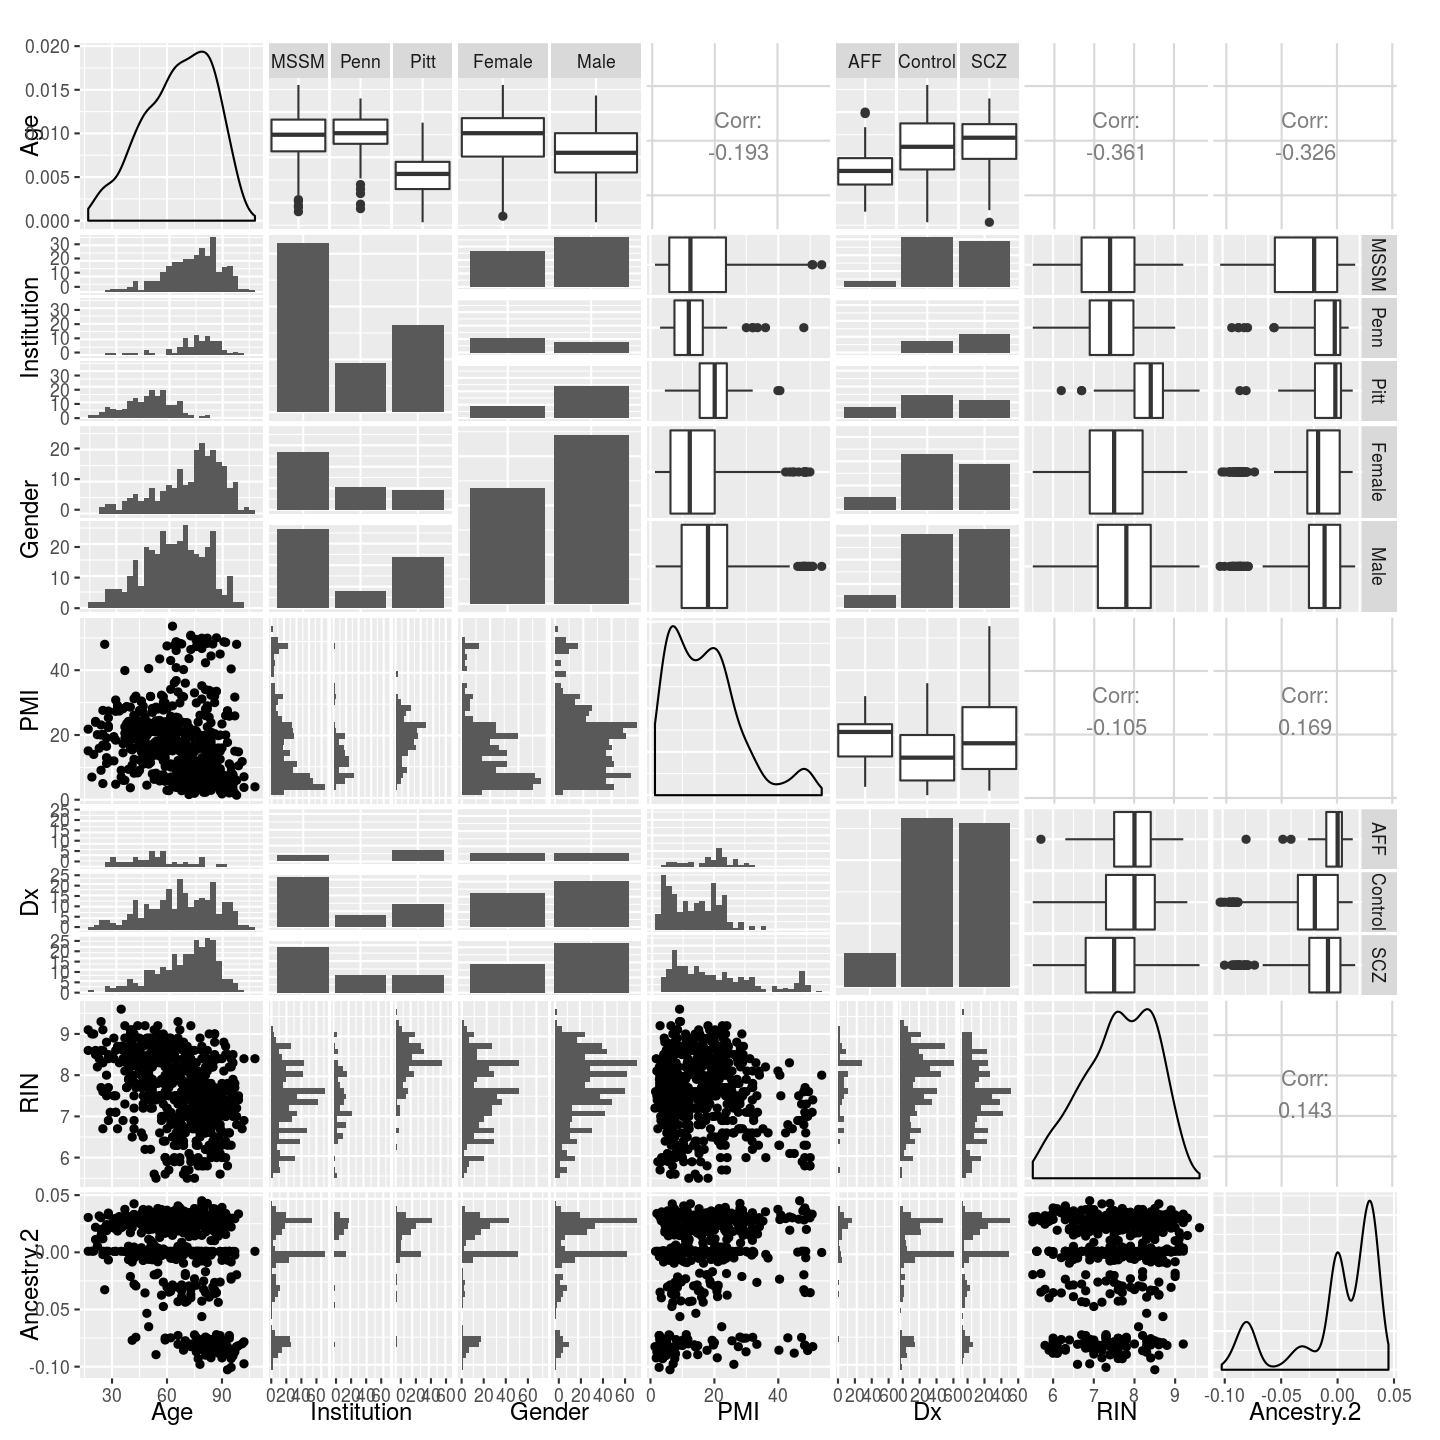
\includegraphics[scale=0.6]{figures/2016-06-26-trellis-display-of-data/evar-scatterplot-matrix-2.png}
\end{center}
\caption{}
\label{fig:predictor-associations}
\end{figure}

\begin{figure}
\begin{center}
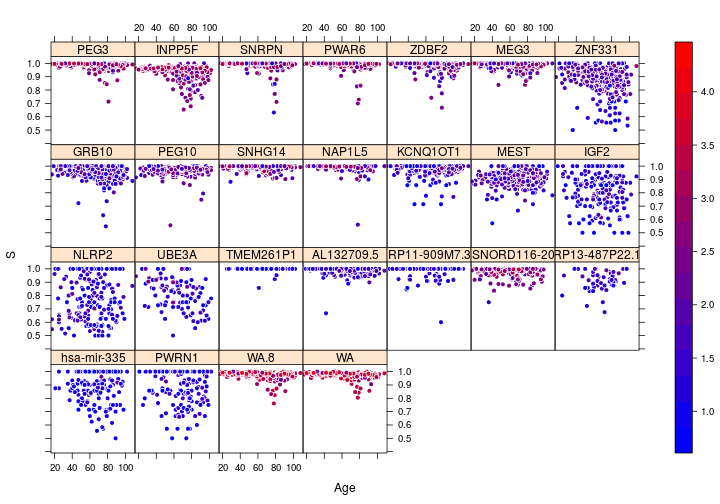
\includegraphics[scale=0.6]{figures/2016-06-26-trellis-display-of-data/S-age-tot-read-count-1.png}
\end{center}
\caption{}
\label{fig:weight-of-evidence}
\end{figure}

\begin{figure}
\begin{center}
\includegraphics[scale=0.6]{figures/2016-08-21-likelihood-surface/ll-surf-coefs-1.png}
\end{center}
\caption{}
\label{fig:likelihood-surface}
\end{figure}

\begin{figure}
\begin{center}
\includegraphics[scale=0.6]{figures/2016-05-07-comparing-regression-models/s-r-stat-nlm-check-peg3-1.pdf}
\end{center}
\caption{}
\label{fig:non-constant-variance}
\end{figure}

\begin{figure}
\begin{center}
\includegraphics[scale=0.6]{figures/2016-06-22-extending-anova/reg-coef-logi-S-1.pdf}
\end{center}
\caption{}
\label{fig:all-effects-logi.S}
\end{figure}

\begin{figure}
\begin{center}
\includegraphics[scale=0.6]{figures/2016-06-22-extending-anova/reg-coef-logi2-S-1.pdf}
\end{center}
\caption{}
\label{fig:all-effects-logi2.S}
\end{figure}

\begin{figure}
\begin{center}
\includegraphics[scale=0.6]{figures/2016-06-22-extending-anova/reg-coef-wnlm-R-1.pdf}
\end{center}
\caption{}
\label{fig:all-effects-wnlm.R}
\end{figure}

\begin{figure}
\begin{center}
\includegraphics[scale=0.6]{figures/2016-06-22-extending-anova/reg-coef-unlm-R-1.pdf}
\end{center}
\caption{}
\label{fig:all-effects-unlm.R}
\end{figure}

\begin{figure}
\begin{center}
\includegraphics[scale=0.6]{figures/2016-06-17-extending-regression-analysis/beta-age-wnlm-R-vs-logi-S-1.pdf}
\end{center}
\caption{}
\label{fig:age-effect-two-model}
\end{figure}

\begin{figure}
\begin{center}
\includegraphics[scale=0.6]{figures/2016-07-08-conditional-inference/beta-age-cond-logi-S-1.pdf}
\end{center}
\caption{}
\label{fig:interaction}
\end{figure}

% Supplementary tables

\setcounter{table}{0}
\makeatletter 
\renewcommand{\thetable}{S\@arabic\c@table}
\makeatother

\end{document}
